\documentclass[aspectratio=169]{beamer}

\mode<presentation>
{
  \setbeamertemplate{background canvas}[square]
  \pgfdeclareimage[width=6em,interpolate=true]{dsailogo}{../dsai-logo}
  \pgfdeclareimage[width=6em,interpolate=true]{erasmuslogo}{../erasmus-logo}
  \titlegraphic{\pgfuseimage{dsailogo} \hspace{0.2in} \pgfuseimage{erasmuslogo}}
  %\usetheme{default}
  \usetheme{Madrid}
  \usecolortheme{rose}
  \usefonttheme[onlysmall]{structurebold}
}

\usepackage{pgf,pgfarrows,pgfnodes,pgfautomata,pgfheaps,pgfshade}
\usepackage{amsmath,amssymb}
\usepackage{graphics}
\usepackage{ragged2e}
\usepackage[latin1]{inputenc}
\usepackage{colortbl}
\usepackage[absolute,overlay]{textpos}
\setlength{\TPHorizModule}{30mm}
\setlength{\TPVertModule}{\TPHorizModule}
\textblockorigin{10mm}{10mm}
\usepackage[english]{babel}
\setbeamercovered{dynamic}

\AtBeginSection[]{
  \begin{frame}<beamer>
  \frametitle{Outline}
  \tableofcontents[currentsection]
  \end{frame}
}

\title[Computer Vision]{Computer Vision\\Projective Geometry}
\author{dsai.asia}
\institute[]{Asia Data Science and Artificial Intelligence Master's Program}
\date{}

% My math definitions

\renewcommand{\vec}[1]{\boldsymbol{#1}}
\newcommand{\mat}[1]{\mathtt{#1}}
\renewcommand{\null}[1]{{\cal N}(#1)}
\def\Rset{\mathbb{R}}
\def\Pset{\mathbb{P}}
\def\norm{\mbox{$\cal{N}$}}
\newcommand{\crossmat}[1]{\begin{bmatrix} #1 \end{bmatrix}_{\times}}
\DeclareMathOperator*{\argmax}{argmax}
\DeclareMathOperator*{\argmin}{argmin}
\DeclareMathOperator*{\sign}{sign}
\DeclareMathOperator*{\trace}{trace}

\newcommand{\stereotype}[1]{\guillemotleft{{#1}}\guillemotright}

\newcommand{\myfig}[3]{\centerline{\includegraphics[width={#1}]{{#2}}}
    \centerline{\scriptsize #3}}

\begin{document}

%%%%%%%%%%%%%%%%%%%%%%%%%%%%%%%%%%%%%%%%%%%%%%%%%%%%%%%%%%%%
%%             CONTENTS START HERE

%\setbeamertemplate{navigation symbols}{}

\frame{\titlepage}

%--------------------------------------------------------------------
%\part<presentation>{Part name}
%
%\frame{\partpage}

\begin{frame}
\frametitle{Readings}

Readings for these lecture notes:
\begin{itemize}
\item[-] Hartley, R., and Zisserman, A. {\em Multiple View Geometry in
    Computer Vision}, Cambridge University Press, 2004, Chapters 1--3.
\item[-] Szeliski, R. \textit{Computer Vision: Algorithms and Applications},
    Springer, 2021.
\end{itemize}

\medskip

These notes contain material $\copyright$ Hartley and Zisserman
(2004) and Szeliski (2021).

\end{frame}

%--------------------------------------------------------------------
\section{2D projective geometry}
%--------------------------------------------------------------------


\begin{frame}
\frametitle{2D projective geometry}
\framesubtitle{Introduction}

We begin with 2D projective geometry because it's simple, then we'll
generalize to 3D.

\medskip

In particular, we consider \alert{what happens when we perform
projective transformations of the plane}.

\medskip

\alert{Projective transformations} model the distortions introduced by
\alert{projective cameras} (more on cameras later).

\medskip

In projective cameras, funny things happen.  Although straight lines
stay straight, parallel lines are no longer parallel.

\medskip

Projective geometry gives us the mathematics for these kinds of
transformations.

\end{frame}

\begin{frame}
\frametitle{2D projective geometry}
\framesubtitle{The 2D projective plane: points in $\Rset^2$}

A \alert{point} in the plane can be represented as a pair $(x,y)$ in
$\Rset^2$.

\medskip

We consider $\Rset^2$ as a vector space and we write the point $(x,y)$
as a vector.

\medskip

This makes it possible to write transformations of points as matrices.

\medskip

Generally, we write transformations on the left and points on the
right, so we need to write points as column vectors, i.e.\ $(x,y)^T$.

\medskip

We will typically write column vectors using bold upright symbols, e.g.,
$\vec{x} = (x,y)^T$.

\end{frame}

\begin{frame}
\frametitle{2D projective geometry}
\framesubtitle{The 2D projective plane: lines in $\Rset^2$}

A \alert{line} in the plane is normally represented by an equation
like $ax+by+c=0$.  The parameters $a$, $b$, and $c$ give us different
lines.

\medskip

This means we can write a line in $\Rset^2$ as the vector $(a,b,c)^T$.

\end{frame}

\begin{frame}
\frametitle{2D projective geometry}
\framesubtitle{The 2D projective plane: homogeneous coordinates and $\Pset^2$}

$(a,b,c)^T$ represents the same line as $k(a,b,c)^T$ for any non-zero
constant $k$.

\medskip

A \alert{homogeneous vector} is an equivalence class of vectors
defined by scaling.

\medskip

The set of homogeneous equivalence classes of vectors in $\Rset^3 -
(0,0,0)^T$ is called the \alert{projective space} $\Pset^2$.

\end{frame}

\begin{frame}
\frametitle{2D projective geometry}
\framesubtitle{The 2D projective plane: homogeneous point representations}

Since a point $\vec{x}=(x,y)^T$ lies on a line $\vec{l}=(a,b,c)^T$ iff
$ax+by+c=0$, we can equivalently write the inner product
$(x,y,1)(a,b,c)^T=(x,y,1)\vec{l}=0$.

\medskip

If $(x,y,1)\vec{l}=0$, it is also true that $(kx,ky,k)\vec{l}=0$.

\medskip

This makes it convenient to represent a point $\vec{x}=(x,y)^T$ in
$\Rset^2$ with the \alert{homogeneous vector} $(x,y,1)^T$.

\medskip

This means the arbitrary point $\vec{x}=(x_1,x_2,x_3)^T$ in $\Pset^2$
can be used to represent the point $(x_1/x_3,x_2/x_3)$ in $\Rset^2$.

\medskip

This is nice!  Why?  Because now we can say that a homogeneous point
$\vec{x} = (x_1,x_2,x_3)^T$ lies on line $\vec{l}$ iff
$\vec{x}^T\vec{l}=0$.

\end{frame}

\begin{frame}
\frametitle{2D projective geometry}
\framesubtitle{The 2D projective plane: intersection of two lines}

Another nice property: the \alert{intersection of two lines}
$\vec{l}$ and $\vec{l}'$ is the point $\vec{x}=\vec{l}\times\vec{l}'$.

\medskip

Reminder: the cross product of two vectors $\vec{x}_1 = (x_1,x_2,x_3)^T$ and
$\vec{x}' = (x_1',x_2',x_3')^T$ is defined as
\begin{equation*}
\vec{x}\times\vec{x}' =
\begin{vmatrix}
\vec{i} & \vec{j} & \vec{k} \\
x_1 & x_2 & x_3 \\
x_1' & x_2' & x_3'
\end{vmatrix}
\end{equation*}

\medskip

Another reminder: if $\vec{x} = \vec{l} \times \vec{l}'$, $\vec{x}$ is
the vector normal to $\vec{l}$ and $\vec{l}'$ with magnitude equal to
the area of the parallelogram formed by $\vec{l}$ and $\vec{l}'$.

\medskip

Proof: Since $\vec{x}$ is orthogonal to both $\vec{l}$ and $\vec{l}'$
we know $\vec{l}^T\vec{x}=0$ and $\vec{l}'^T\vec{x}=0$, meaning
$\vec{x}$ lies on both $\vec{l}$ and $\vec{l}'$!

\medskip

Similarly, the line $\vec{l}$ joining two points is just
$\vec{l}=\vec{x}\times\vec{x}'$.

\end{frame}

\begin{frame}
\frametitle{2D projective geometry}
\framesubtitle{Ideal points and the line at infinity}

Where do the parallel lines $(a,b,c)^T$ and $(a,b,c')^T$ intersect?

\medskip

The cross product turns out to be $(c'-c)(b,-a,0)^T = (b,-a,0)^T$ in
$\Pset^2$ but this point has no inhomogeneous representation. (What is
$(b/0,-a/0)^T$?)

\medskip

We call such a point $(x_1,x_2,0)^T$ in $\Pset^2$ an \alert{ideal
point} or a \alert{point at infinity} along the direction
$(x_1,x_2)^T$.

\medskip

All points at infinity lie on the \alert{line at infinity}
$\vec{l}_{\infty} = (0,0,1)^T$ (remember that lines in $\Pset^2$
correspond to planes in $\Rset^3$, points at infinity lie on the plane
$x_3=0$, so we represent the plane $x_3=0$ by its normal vector
$(0,0,1)^T$).

\medskip

In $\Pset^2$, then, we can say that any two lines intersect, even if
they are parallel.

\end{frame}

\begin{frame}
\frametitle{2D projective geometry}
\framesubtitle{A model for the projective plane}

Here's how to think of $\Pset^2$: it is a \alert{set of rays}
through the origin in $\Rset^3$.

\medskip

If we consider all vectors $k(x_1,x_2,x_3)^T$ as $k$ varies, we obtain
a ray through the origin.  Each such ray is a \alert{single point} in
$\Pset^2$.

\medskip

A \alert{line} between any two different points in $\Pset^2$ forms a
\alert{plane through the origin}.

\medskip

Inhomogeneous representations of points and lines can be obtained by
finding the intersection of their rays and planes with the plane
$x_3=1$.

\end{frame}

\begin{frame}
\frametitle{2D projective geometry}
\framesubtitle{A model for the projective plane}

\myfig{3in}{HZ-fig1-1}{Hartley and Zisserman (2004), Fig.\ 2.1}

\end{frame}

\begin{frame}
\frametitle{2D projective geometry}
\framesubtitle{A model for the projective plane}

In $\Rset^3$, \alert{lines} through the origin that lie
in the $x_1x_2$ plane
represent \alert{ideal points} in $\Pset^2$.

\medskip

\alert{All other lines} through the origin represent \alert{points} in
$\Pset^2$.

\medskip

\alert{Planes} through the origin in $\Rset^3$ represent \alert{lines} in
$\Pset^2$.

\medskip

The vector $(a,b,c)^T$ representing a line in the Euclidean plane,
when interpreted as a vector in $\Rset^3$, is \alert{orthogonal
to the $\Rset^3$ plane representing the line in $\Pset^2$}.

\medskip

You should try to prove that this must be so.

\end{frame}


\begin{frame}
\frametitle{2D projective geometry}
\framesubtitle{Conics}

\alert{Conic sections} or just \alert{conics} are curves in the plane
described by 2nd-degree equations.

\medskip

In Euclidean geometry, conics can be parabolas, hyperbolas, and
ellipses, or ``degenerate'' conics (two lines or a single line).

\medskip

In inhomogeneous coordinates, we write conics as
\begin{equation*}
ax^2 + bxy + cy^2 + dx + ey + f = 0
\end{equation*}

\medskip

We homogenize the equation by replacing $x$ by $x_1/x_3$ and $y$ by
$x_2/x_3$.  This gives us
\begin{equation*}
ax_1^2 + bx_1x_2 + cx_2^2 + dx_1x_3 + ex_2x_3 + fx_3^2 = 0
\end{equation*}

\end{frame}

\begin{frame}
\frametitle{2D projective geometry}
\framesubtitle{Conics}

With homogeneous points, similar to the point-line equation, conics
can be written in matrix form:
\begin{equation*}
\vec{x}^T\mat{C}\vec{x}=0
\end{equation*}

\medskip

Where the (symmetric) conic coefficient matrix $\mat{C}$ is given by
\begin{equation*}
\mat{C}=\begin{bmatrix}
a & b/2 & d/2 \\
b/2 & c & e/2 \\
d/2 & e/2 & f \end{bmatrix}
\end{equation*}

\medskip

$\mat{C}$ is \alert{homogeneous} because scaling by a non-zero
constant does not change the conic.

\medskip

$\mat{C}$ has five degrees of freedom, and each point on the conic
gives us one equation linear in the conic's parameters, so we need
five points to uniquely define a conic up to scale.

\end{frame}

\begin{frame}
\frametitle{2D projective geometry}
\framesubtitle{Conics}

If we find the points $\vec{x}$ satisfying
$\vec{x}^T\mat{C}\vec{x}=0$, we obtain the plane curve described by
$\mat{C}$:

\medskip

\myfig{1.9in}{HZ-fig1-2a}{\begin{minipage}{2.5in} \centering Solution of
    $\vec{x}^T\mat{C}\vec{x}=0$\\
Hartley and Zisserman (2004), Fig.\ 2.2(a) \end{minipage}}

\medskip

\alert{Exercise}: write the circle about the origin with radius $r$ in conic
matrix form, and verify that the points on the circle satisfy
$\vec{x}^T\mat{C}\vec{x}=0$.

\end{frame}


\begin{frame}
\frametitle{2D projective geometry}
\framesubtitle{Conics}

\begin{columns}

\column{2.2in}

What happens if we take an arbitrary point $\vec{x}$ on the conic and
compute $\mat{C}\vec{x}$, treating $\mat{C}$ as a \alert{linear
  operator}?

\medskip

We obtain a 3-vector whose inner product with $\vec{x}$ is 0.  This
means that $\vec{l}=\mat{C}\vec{x}$ necessarily represents a
\alert{line passing through $\vec{x}$}.

\medskip

In fact, the resulting line is special: it is the \alert{tangent} to
the conic at $\vec{x}$.

\column{2.3in}

\myfig{1.9in}{HZ-fig1-2b}{
  \parbox{2.3in}{
    \begin{center}
      The line $\vec{l}=\mat{C}\vec{x}$ is the tangent to $\mat{C}$
      through $\vec{x}$.\\
      \mbox{\hspace{0.2in}} \\
      Hartley and Zisserman (2004), Fig. 2.2(b) \end{center}}}

\end{columns}

\end{frame}

\begin{frame}
\frametitle{2D projective geometry}
\framesubtitle{Projective transformations}

There is an important class of transformations on $\Pset^2$ called
\alert{projectivities} or \alert{homographies} or
\alert{collineations}.

\medskip

A projectivity (homography) is a transform that can be represented by
a 3$\times$3 non-singular matrix $\mat{H}$.

\medskip

Homographies are \alert{linear mappings} of homogeneous coordinates:
\begin{equation*}
\begin{pmatrix}
x_1' \\ x_2' \\ x_3'
\end{pmatrix} =
\begin{bmatrix}
h_{11} & h_{12} & h_{13} \\
h_{21} & h_{22} & h_{23} \\
h_{31} & h_{32} & h_{33}
\end{bmatrix}
\begin{pmatrix}
x_1 \\ x_2 \\ x_3
\end{pmatrix}
\end{equation*}
or simply $\vec{x}' = \mat{H}\vec{x}$.

\medskip

Since scaling $\mat{H}$ doesn't change the result, we say $\mat{H}$ is
a \alert{homogeneous matrix} with 8 degrees of freedom.

\end{frame}

\begin{frame}
\frametitle{2D projective geometry}
\framesubtitle{Projective transformations as central projections}

Homographies can also be thought of as \alert{central projections}
mapping one plane to another:

\myfig{3in}{HZ-fig1-3}{Hartley and Zisserman (2004), Fig.\ 2.3}

\medskip

[Actually, central projections between rectilinear coordinate systems
as shown here are called \alert{perspectivities} and only have 6
degrees of freedom.]

\end{frame}

\begin{frame}
\frametitle{2D projective geometry}
\framesubtitle{Projective transformations: rectification}

One application of homographies is \alert{rectification}.  As an
example, suppose we want to remove projective distortion from a
perspective image of a plane:

\begin{columns}
\column{2in}
\myfig{1.9in}{HZ-fig1-4a}{(a)}
\column{2in}
\myfig{1.9in}{HZ-fig1-4b}{(b)}
\end{columns}
\centerline{Hartley and Zisserman (2004), Fig. 2.4}

\end{frame}

\begin{frame}
\frametitle{2D projective geometry}
\framesubtitle{Projective transformations: rectification}

By picking any four points in an original image and the desired
corresponding points in the new image, we obtain 8 linear equations in
the 9 unknowns of $\mat{H}$, allowing us to compute the parameters of
$\mat{H}$:

\begin{columns}
\column{2in}
\begin{equation*}
x' = \frac{x_1'}{x_3'} =
\frac{h_{11}x+h_{12}y+h_{13}}{h_{31}x+h_{32}y+h_{33}},
\end{equation*}
\column{2in}
\begin{equation*}
y' = \frac{x_2'}{x_3'} =
\frac{h_{21}x+h_{22}y+h_{23}}{h_{31}x+h_{32}y+h_{33}}.
\end{equation*}
\end{columns}

\bigskip

\bigskip

See the example \texttt{compute\_homography.m} that implements this
idea.

\end{frame}

\begin{frame}
\frametitle{2D projective geometry}
\framesubtitle{Projective transformations: examples}

Here are a few of the most important examples of homographies (Hartley
and Zisserman, 2004, Fig. 2.5):

\begin{columns}
\column{1.5in}
\myfig{1.4in}{HZ-fig1-5a}{}
\column{1.5in}
\myfig{1.4in}{HZ-fig1-5b}{}
\column{1.5in}
\myfig{1.2in}{HZ-fig1-5c}{}
\end{columns}

\vspace{-.1in}

{\scriptsize \begin{columns}[T]
\column{1.5in}
\centerline{\parbox{1.4in}{Images of a plane from two
    cameras related by a rotation and a translation.}}
\column{1.5in}
\centerline{\parbox{1.4in}{Images of arbitrary objects
    from two cameras related by a rotation.}}
\column{1.5in}
\centerline{\parbox{1.4in}{Images of shadows of planar objects.}}
\end{columns}}

\bigskip

Note that images of \alert{arbitrary} objects from two cameras related
by a rotation and translation are \alert{not} related by homographies.

\end{frame}

\begin{frame}
\frametitle{2D projective geometry}
\framesubtitle{Projective transformations: examples}

Given a point homography $\vec{x}'=\mat{H}\vec{x}$:
\begin{itemize}
\item The corresponding \alert{line homography} is
  $\vec{l}'=\mat{H}^{-T}\vec{l}$
\item The corresponding \alert{conic homography} is
  $\mat{C}'=\mat{H}^{-T}\mat{C}\mat{H}^{-1}$
\end{itemize}

\end{frame}

\begin{frame}
\frametitle{2D projective geometry}
\framesubtitle{A hierarchy of transformations}

We can create a \alert{hierarchy of transformations} based on the
restrictions that we put on a linear transformation $\mat{H}$.

\medskip

The \alert{real linear group} $GL(3)$ consists of all invertible real
$3\times 3$ matrices.\footnote{Recall that a \alert{group} is a set
  paired with an operation that has an inverse, associativity, an
  identity, and closure.}

\medskip

When we place all members of $GL(3)$ related by
scale in an equivalence class, we obtain the \alert{projective linear
group} $PL(3)$.

\medskip

There are three important subgroups of $PL(3)$:
\begin{itemize}
\item The \alert{affine} group in which the bottom row is constrained to
  $(0,0,1)$;
\item The \alert{similarity} group in which the rows and columns
  of the upper-left 2$\times$2 submatrix are orthogonal;
\item The \alert{Euclidean} or \alert{isometry} group in which the
  upper-left 2$\times$2 submatrix is orthonormal.
\end{itemize}

\end{frame}

\begin{frame}
\frametitle{2D projective geometry}
\framesubtitle{A hierarchy of transforms}

{\small
\begin{tabular}{cccc}
\hline
\hline
Group & Matrix & Distortion & Invariant properties \\
\hline
\begin{minipage}{0.5in} Projective 8~dof \end{minipage} &
$\begin{bmatrix}h_{11} & h_{12} & h_{13} \\
                h_{21} & h_{22} & h_{23} \\
                h_{31} & h_{32} & h_{33} \end{bmatrix}$ &
\parbox{0.5in}{\centerline{
\includegraphics[height=0.6in]{xform1}}} &
\begin{minipage}{1.8in} Concurrency, collinearity, order of contact,
  tangent discontinuities and cusps, cross ratios \end{minipage} \\
\hline
\begin{minipage}{0.5in} Affine 6~dof \end{minipage} &
$\begin{bmatrix}a_{11} & a_{12} & t_x \\
                a_{21} & a_{22} & t_y \\
                0 & 0 & 1 \end{bmatrix}$ &
\parbox{0.5in}{\centerline{
\includegraphics[height=0.6in]{xform2}}} &
\begin{minipage}{1.8in} Parallelism, ratio of areas, ratio of lengths
  on collinear or parallel lines, linear combinations of vectors, the
  line at infinity $\vec{l}_{\infty}$\end{minipage} \\
\hline
\begin{minipage}{0.5in} Similarity 4~dof \end{minipage} &
$\begin{bmatrix}sr_{11} & sr_{12} & t_x \\
                sr_{21} & sr_{22} & t_y \\
                0 & 0 & 1 \end{bmatrix}$ &
\parbox{0.5in}{\centerline{
\includegraphics[height=0.6in]{xform3}}} &
\begin{minipage}{1.8in} Ratio of lengths, angle \end{minipage} \\
\hline
\begin{minipage}{0.5in} Euclidean 3~dof \end{minipage} &
$\begin{bmatrix}r_{11} & r_{12} & t_x \\
                r_{21} & r_{22} & t_y \\
                0 & 0 & 1 \end{bmatrix}$ &
\parbox{0.5in}{\centerline{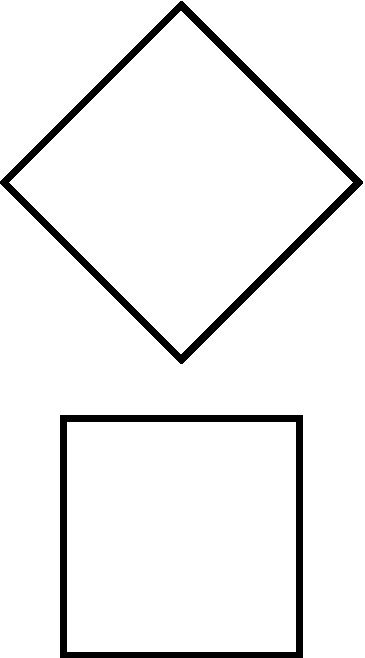
\includegraphics[height=0.6in]{xform4}}} &
\begin{minipage}{1.8in} Length, area\end{minipage} \\
\hline
\hline
\end{tabular}}

\centerline{\scriptsize Hartley and Zisserman (2004), Table 2.1}

\end{frame}

\begin{frame}
\frametitle{2D projective geometry}
\framesubtitle{Action of projectivities and affinities on ideal points}

What happens when we apply a homography $\mat{H}$ to a point at
infinity?

\medskip

Affinities map ideal points to ideal points:
\begin{equation*}
\begin{bmatrix}
\mat{A} & \vec{t} \\
\vec{0}^T & 1 \\
\end{bmatrix}
\begin{pmatrix}
x_1 \\ x_2 \\ 0
\end{pmatrix}
=
\begin{pmatrix}
\mat{A} \begin{pmatrix} x_1 \\ x_2 \end{pmatrix}\\
0
\end{pmatrix}
\end{equation*}
but general projectivities can map ideal points to finite points:
\begin{equation*}
\begin{bmatrix}
\mat{A} & \vec{t} \\
\vec{v}^T & 1 \\
\end{bmatrix}
\begin{pmatrix}
x_1 \\ x_2 \\ 0
\end{pmatrix}
=
\begin{pmatrix}
\mat{A} \begin{pmatrix} x_1 \\ x_2 \end{pmatrix}\\
v_1 x_1 + v_2 x_2
\end{pmatrix}
\end{equation*}

\end{frame}

\begin{frame}
\frametitle{2D projective geometry}
\framesubtitle{Action of projectivities and affinities on ideal points}

\begin{columns}
\column{1.5in}
\myfig{1.4in}{HZ-fig1-6a}{}
\column{1.5in}
\myfig{1.4in}{HZ-fig1-6b}{}
\column{1.5in}
\myfig{1.4in}{HZ-fig1-6c}{}
\end{columns}

\begin{columns}[T]
\column{1.5in}
\parbox{1.4in}{Similarity: circularity is invariant}
\column{1.5in}
\parbox{1.4in}{Affinity: parallelism is invariant}
\column{1.5in}
\parbox{1.4in}{Projectivity: the line at infinity becomes finite
  (parallel lines on the plane intersect at finite points on
  $\vec{l}_{\infty}$)}
\end{columns}

\centerline{\scriptsize Hartley and Zisserman (2004), Fig. 2.6}

\end{frame}

%--------------------------------------------------------------------
\section{3D projective geometry}
%--------------------------------------------------------------------

\begin{frame}
\frametitle{3D projective geometry}
\framesubtitle{Introduction}

Now we move to \alert{projective 3-space}, or $\Pset^3$.

\medskip

Things will mostly generalize from $\Pset^2$.

\medskip

We'll use homogeneous coordinates in $\Rset^4$ to represent points
\alert{and planes} in $\Pset^3$.

\medskip

We'll see that parallel lines and parallel planes intersect on the
\alert{plane at infinity} $\vec{\pi}_{\infty}$.

\end{frame}

\begin{frame}
\frametitle{3D projective geometry}
\framesubtitle{Points in $\Pset^3$}

We represent a 3D point $(X,Y,Z)^T$ in homogeneous coordinates
$\vec{X}=(X_1,X_2,X_3,X_4)^T$ with $X_4\not=0$ and
\[ X=X_1/X_4, Y=X_2/X_4, Z=X_3/X_4.\]

\medskip

Homogeneous coordinates with $X_4=0$ represent \alert{points at
infinity}.

\medskip

A \alert{projective transformation on $\Pset^3$} is a linear
transformation on homogeneous 4-vectors, represented by a non-singular
4$\times$4 matrix: $\vec{X}' = \mat{H}\vec{X}$.

\medskip

$\mat{H}$ is homogeneous and in general has 15 degrees of freedom.

\end{frame}

\begin{frame}
\frametitle{3D projective geometry}
\framesubtitle{Planes in $\Pset^3$}

Whereas points and lines are dual in $\Pset^2$, \alert{points and
planes} are dual in $\Pset^3$.

\medskip

A plane in 3-space is written
\begin{equation*}
\pi_1 X + \pi_2 Y + \pi_3 Z + \pi_4 = 0.
\end{equation*}

\medskip

The equation is unaffected by scalar multiplication, so we can
represent a plane as the \alert{homogeneous vector}
$(\pi_1,\pi_2,\pi_3,\pi_4)^T$.

\medskip

Homogenizing the point $\vec{X}$, we get \[ \pi_1 X_1 + \pi_2 X_2 +
\pi_3 X_3 + \pi_4 X_4 = 0 \] or simply $\vec{\pi}^T\vec{X}=0$ to
express that the point $\vec{X}$ lies on the plane $\vec{\pi}$.

\end{frame}

\begin{frame}
\frametitle{3D projective geometry}
\framesubtitle{Points and planes in $\Pset^3$}

Suppose we have 3 points in general position.  We can find the plane
they lie in by constructing the equation
\begin{equation*}
\mat{X}\vec{\pi} =
\begin{bmatrix} \vec{X}_1^T \\ \vec{X}_2^T \\ \vec{X}_3^T
\end{bmatrix}
\vec{\pi} = \vec{0}
\end{equation*}

\medskip

As long as the 3$\times$4 matrix $\mat{X}$ has rank\footnote{The rank
  of matrix $\mat{A}$ is the number of linearly independent rows or
  columns in $\mat{A}$.} 3, the solution
$\vec{\pi}$ is the \alert{right null space}\footnote{The
right null space of matrix $\mat{A}$, written $\null{\mat{A}}$, is the
set of all solutions of $\mat{A}\vec{x}=\vec{0}$.} of $\mat{X}$.

\medskip

If $\mat{X}$ is rank 2, we have collinear points and the equation
defines a \alert{pencil of planes}\footnote{Just a fancy term for the
set of planes intersecting at a given line.} with the line of
collinear points as its axis.

\end{frame}

\begin{frame}
\frametitle{3D projective geometry}
\framesubtitle{Points and planes in $\Pset^3$}

Analogous to the definition of the line through two points in
$\Pset^2$, the plane through three points in $\Pset^3$ can be written
in terms of determinants and minors.

\medskip

We finally obtain (see text for proof)
\[ \vec{\pi} =
  \begin{pmatrix}
    (\tilde{\vec{X}}_1 - \tilde{\vec{X}}_3) \times
    (\tilde{\vec{X}}_2 - \tilde{\vec{X}}_3) \\
    -\tilde{\vec{X}}_3^T (\tilde{\vec{X}}_1 \times \tilde{\vec{X}}_2)
  \end{pmatrix}
\]

where $\tilde{\vec{X}}$ is the inhomogeneous representation of point
$\vec{X}$.

\medskip

So we can find the plane through three points by finding $\null{\mat{X}}$ or
by using some vector algebra.

\end{frame}

\begin{frame}
\frametitle{3D projective geometry}
\framesubtitle{Lines in $\Pset^3$}

Lines in 3-space can be defined by their \alert{intersection with two
given planes}:

\myfig{2.0in}{HZ-fig2-1}{Hartley and Zisserman (2004) Fig.\ 3.1}

\medskip

This means a line in 3-space has \alert{4 degrees of freedom}.

\medskip

Wouldn't it be natural to represent lines as 5-element homogeneous
vectors?

\medskip

Unfortunately this doesn't work well with 4-vectors for lines and
planes.

\medskip

Several alternative representations for lines have been proposed.

\end{frame}

\begin{frame}
\frametitle{3D projective geometry}
\framesubtitle{Lines in $\Pset^3$: homogeneous point representation}

In the \alert{homogeneous point representation} of a line, given two
homogeneous points $\vec{A}$ and $\vec{B}$ on the line, we write
\begin{equation*}
\mat{W} = \begin{bmatrix} \vec{A}^T \\ \vec{B}^T \end{bmatrix},
\end{equation*}
in which case:
\begin{itemize}
\item The \alert{span}\footnote{The set of all linear combinations of
    the columns of a matrix.} of $\mat{W}^T$ is the \alert{pencil of
    points}\footnote{Just a fancy term for the set of points on a
    line.}  $\lambda \vec{A} + \mu \vec{B}$ on the line.\footnote{To
    convince yourself of this, consider the inhomogeneous parametric
    representation of the line
    $\tilde{\vec{A}}+t(\tilde{\vec{B}}-\tilde{\vec{A}})$ with
    $t=\frac{\mu}{\lambda+\mu}$.}
\item The span of the 2-dimensional right \alert{null-space} of
  $\mat{W}$ is the \alert{pencil of planes} with the line as the axis.
\end{itemize}

\end{frame}

\begin{frame}
\frametitle{3D projective geometry}
\framesubtitle{Lines in $\Pset^3$: dual homogeneous plane representation}

There is a dual representation of a line as the \alert{intersection of two
planes} $\vec{P}$ and $\vec{Q}$:
\begin{equation*}
\mat{W}^* = \begin{bmatrix} \vec{P}^T \\ \vec{Q}^T \end{bmatrix}
\end{equation*}
in this representation,
\begin{itemize}
\item The \alert{span} of $\mat{W}^{*T}$ is the \alert{pencil of
  planes} $\lambda'\vec{P} + \mu'\vec{Q}$ with the line as an axis.
\item The span of the 2-dimensional \alert{null-space} of $\mat{W}^*$
  is the \alert{pencil of points} on the line.
\end{itemize}

\medskip

Example: find $\mat{W}$ and $\mat{W}^*$ for the points
$(1,0,0,1)^T$ and $(2,0,0,1)^T$
and verify that $\mat{W}^*\mat{W}^T=\mat{W}\mat{W}^{*T}=\mat{0}$.

\end{frame}

\begin{frame}
\frametitle{3D projective geometry}
\framesubtitle{Lines in $\Pset^3$: Pl\"ucker matrix representation}

We can also represent a line through $\vec{A}$ and $\vec{B}$ by a
4$\times$4 \alert{skew-symmetric}\footnote{Recall that a skew-symmetric matrix
is a matrix $\mat{A}$ such that $\mat{A}^T=-\mat{A}$.} homogeneous
matrix $\mat{L}$ defined by \[ l_{ij} = A_iB_j - B_iA_j \] or
equivalently,
\begin{equation*}
\mat{L} = \vec{A}\vec{B}^T - \vec{B}\vec{A}^T.
\end{equation*}

\medskip

$\mat{L}$ is the \alert{Pl\"ucker} matrix representation of a line.

\end{frame}

\begin{frame}
\frametitle{3D projective geometry}
\framesubtitle{Lines in $\Pset^3$: Pl\"ucker matrix representation}

Some nice properties of $\mat{L}$:
\begin{itemize}
\item The rank of $\mat{L}$ is 2 and its 2-dimensional null-space is
  spanned by the pencil of planes with the line as an axis
  ($\mat{L}\mat{W}^{*T} = \mat{0}$).
\item $\mat{L}$ has 4 degrees of freedom, the same as a line, since it
  is skew-symmetric (having only 6 independent non-zero elements),
  homogeneous, and constrained so that $\det\mat{L}=0$ (its rank is
  2).
\item The relation $\mat{L}=\vec{A}\vec{B}^T-\vec{B}\vec{A}^T$ is the
  generalization to $\Pset^3$ of the relation
  $\vec{l}=\vec{x}\times\vec{y}$ of $\Pset^2$.
\item $\mat{L}$ is independent of the points $\vec{A}$ and $\vec{B}$.
\item Under the point transformation $\vec{X}'=\mat{H}\vec{X}$, the
  matrix $\mat{L}$ transforms as $\mat{L}'=\mat{H}\vec{L}\mat{H}^T$.
\end{itemize}

\medskip

Example: write the line through $(1,0,0,1)$ and $(2,0,0,1)$ as
a Pl\"ucker matrix.

\end{frame}

\begin{frame}
\frametitle{3D projective geometry}
\framesubtitle{Lines in $\Pset^3$: dual Pl\"ucker matrix representation}

A \alert{dual} Pl\"ucker representation can be obtained using the
\alert{intersection of two planes} $\vec{P}$ and $\vec{Q}$:
\begin{equation*}
\mat{L}^* = \vec{P}\vec{Q}^T - \vec{Q}\vec{P}^T
\end{equation*}

$\mat{L}^*$ can be derived directly from $\mat{L}$ by a simple rewrite
rule (see text).

\end{frame}

\begin{frame}
\frametitle{3D projective geometry}
\framesubtitle{Lines in $\Pset^3$: dual Pl\"ucker matrix representation}

The advantage of the Pl\"ucker matrix and dual Pl\"ucker matrix
representations is that \alert{joins} and \alert{indicence} properties
are easily represented:
\begin{itemize}
\item The \alert{plane} defined by the \alert{join of a point}
  $\vec{X}$ and \alert{a line} $\mat{L}$ is
  $\vec{\pi}=\mat{L}^*\vec{X}$, and $\mat{L}^*\vec{X}=\vec{0}$ iff
  $\vec{X}$ is on $\mat{L}$.
\item The \alert{point} defined by the \alert{intersection of a line}
  $\mat{L}$ and \alert{a plane} $\vec{\pi}$ is $\vec{X} =
  \mat{L}\vec{\pi}$, and $\mat{L}\vec{\pi} = \vec{0}$ iff $\mat{L}$ is
  on $\vec{\pi}$.
\end{itemize}

\medskip

Example: find the intersection of the line through $(1,0,0,1)$ and
$(2,0,0,1)$ with the plane $X=1$
(note that the plane $X=1$ is represented as $(1,0,0,-1)^T$).

\end{frame}

\begin{frame}
\frametitle{3D projective geometry}
\framesubtitle{Lines in $\Pset^3$: Pl\"ucker line coordinates}

A line can also be represented by the \alert{6 independent non-zero
elements of the skew-symmetric Pl\"ucker matrix} $\mat{L}$.

\medskip

This representation is called the \alert{Pl\"ucker line coordinate
  representation} of a line.

\medskip

See the text for the properties of this representation.

\end{frame}

\begin{frame}
\frametitle{3D projective geometry}
\framesubtitle{Quadrics and dual quadrics}

A \alert{quadric} is the 3D analog of a conic, defined by
\begin{equation*}
\vec{X}^T \mat{Q} \vec{X} = 0
\end{equation*}
where $\mat{Q}$ is a symmetric 4$\times$4 matrix.

\medskip

Here are some properties of quadrics:
\begin{itemize}
\item 9 degrees of freedom (10 independent elements, one lost to
  scale)
\item Defined by 9 points in general position
\item If $\mat{Q}$ is singular, the quadric is \alert{degenerate} and
  can be described by fewer points
\item $\vec{\pi}=\mat{Q}\vec{X}$ is the \alert{polar plane} of
  $\vec{X}$ with respect to $\mat{Q}$.  If $\vec{X}$ is outside
  $\mat{Q}$ then $\vec{\pi}$ is defined by the points of contact of
  the rays through $\vec{X}$ tangent to $\mat{Q}$; if $\vec{X}$ is on
  $\mat{Q}$ then $\vec{\pi}$ is the tangent plane to $\mat{Q}$ at
  $\vec{X}$.
\item The intersection of a plane $\vec{\pi}$ and a quadric $\mat{Q}$
  is always a conic $\mat{C}$.
\item Given a 3D homography $\vec{X}'=\mat{H}\vec{X}$, the quadric
  $\mat{Q}$ transforms as \[ \mat{Q}' =
  \mat{H}^{-T}\mat{Q}\mat{H}^{-1} \]
\end{itemize}

\end{frame}

\begin{frame}
\frametitle{3D projective geometry}
\framesubtitle{Quadrics and dual quadrics}

The dual of a point quadric is an equation on planes: the tangent
planes $\vec{\pi}$ to point quadric $\mat{Q}$ satisfying
$\mat{\pi}^T\mat{Q}^*\mat{\pi} = 0$.

\medskip

Here $\mat{Q}^*=\mat{Q}^{-1}$ if $\mat{Q}$ is invertible, or
$\mat{Q}^*= \textrm{adjoint } \mat{Q}$ otherwise.\footnote{For the
  curious, the adjoint of matrix $\mat{M}$ is defined as the transpose
  of the matrix where element $ij$ is $(-1)^{i+j} \det
  \hat{\mat{M}}_{ij}$ where $\hat{\mat{M}}_{ij}$ is obtained from
  $\mat{M}$ by striking out the $i$-th row and $j$-th column.}

\medskip

Dual quadrics transform as
\[ \mat{Q}^{*\prime} = \mat{H}\mat{Q}^* \mat{H}^T. \]

\end{frame}

\begin{frame}
\frametitle{3D projective geometry}
\framesubtitle{Types of quadrics}

Depending on the rank and signs of the singular values of $\mat{Q}$,
we obtain a variety of different topologies:
\begin{columns}
\column{1in}
\myfig{1in}{HZ-fig2-2a}{}
\column{1in}
\myfig{1in}{HZ-fig2-2b}{}
\column{1in}
\myfig{1in}{HZ-fig2-2c}{}
\column{1in}
\myfig{1in}{HZ-fig2-2d}{}
\end{columns}

\centerline{\scriptsize \parbox{4in}{
  Quadrics projectively equivalent to a spheres (ellipsoid,
  hyperboloid of two sheets, parabaloid), also called \alert{non-ruled
    quadrics}, Hartley and Zisserman (2004), Fig.\ 3.2}}

\end{frame}

\begin{frame}
\frametitle{3D projective geometry}
\framesubtitle{Types of quadrics}

\begin{columns}
\column{2in}
\myfig{2in}{HZ-fig2-3a}{}
\column{2in}
\myfig{2in}{HZ-fig2-3b}{}
\end{columns}
\centerline{\scriptsize
  Hyperboloids of one sheet, also called \alert{ruled quadrics},
  Hartley and Zisserman (2004), Fig.\ 3.3}

\end{frame}

\begin{frame}
\frametitle{3D projective geometry}
\framesubtitle{Types of quadrics}

\begin{columns}
\column{2in}
\myfig{2in}{HZ-fig2-4a}{}
\column{2in}
\myfig{2in}{HZ-fig2-4b}{}
\end{columns}
\centerline{\scriptsize Degenerate quadrics, Hartley and Zisserman
  (2004), Fig.\ 3.4}

\end{frame}

\begin{frame}
\frametitle{3D projective geometry}
\framesubtitle{Twisted cubics}

Conics in 2D can be expressed parametrically in $\Pset^2$ as
\begin{equation}
\begin{pmatrix} x_1 \\ x_2 \\ x_3 \end{pmatrix} =
\mat{A} \begin{pmatrix} 1 \\ \theta \\ \theta^2 \end{pmatrix}
\end{equation}

\medskip

By analogy, various kinds of space curves called \alert{twisted
cubics} can be epressed parametrically in $\Pset^3$ as
\begin{equation}
\begin{pmatrix} X_1 \\ X_2 \\ X_3 \\ X_4 \end{pmatrix} =
\mat{A} \begin{pmatrix} 1 \\ \theta \\ \theta^2 \\ \theta^3 \end{pmatrix}
\end{equation}

\medskip

\end{frame}

\begin{frame}
\frametitle{3D projective geometry}
\framesubtitle{Twisted cubics}

Some views of a twisted cubic:
\begin{columns}
\column{1.3in}
\myfig{1.3in}{HZ-fig2-5a}{}
\column{1.3in}
\myfig{1.3in}{HZ-fig2-5b}{}
\column{1.3in}
\myfig{1.3in}{HZ-fig2-5c}{}
\end{columns}
\centerline{Hartley and Zisserman (2004), Fig.\ 3.5}

\end{frame}

\begin{frame}
\frametitle{3D projective geometry}
\framesubtitle{Hierarchy of transforms}

As we saw in 2D, 3D homographies form a hierarchy from most general to
most constrained:

{\small
\begin{tabular}{cccc}
\hline
\hline
Group & Matrix & Distortion & Invariant properties \\
\hline
\begin{minipage}{0.5in} Projective 15~dof \end{minipage} &
$\begin{bmatrix}\mat{A} & \vec{t} \\
                \vec{v}^T & v \\ \end{bmatrix}$ &
\parbox{0.5in}{\centerline{\includegraphics[height=0.6in]{xform3-1}}} &
\begin{minipage}{1.8in} Intersection and tangency of surfaces in contact.
Sign of Gaussian curvature. \end{minipage} \\
\hline
\begin{minipage}{0.5in} Affine 12~dof \end{minipage} &
$\begin{bmatrix}\mat{A} & \vec{t} \\
                \vec{0}^T & 1 \end{bmatrix}$ &
\parbox{0.5in}{\centerline{\includegraphics[height=0.5in]{xform3-2}}} &
\begin{minipage}{1.8in} Parallelism of planes, volume ratios,
  centroids.  The plane at inifinty $\vec{\pi}_{\infty}$ \end{minipage} \\
\hline
\begin{minipage}{0.5in} Similarity 7~dof \end{minipage} &
$\begin{bmatrix}s\mat{R} & \vec{t} \\
                \vec{0}^T & 1 \end{bmatrix}$ &
\parbox{0.5in}{\centerline{\includegraphics[height=0.4in]{xform3-3}}} &
\begin{minipage}{1.8in} The absolute conic $\mat{\Omega}_{\infty}$.
 \end{minipage} \\
\hline
\begin{minipage}{0.5in} Euclidean 6~dof \end{minipage} &
$\begin{bmatrix} \mat{R} & \vec{t} \\
                \vec{0}^T & 1 \end{bmatrix}$ &
\parbox{0.5in}{\centerline{\includegraphics[height=0.6in]{xform3-3}}} &
\begin{minipage}{1.8in} Volume \end{minipage} \\
\hline
\hline
\end{tabular}}

\centerline{\scriptsize Hartley and Zisserman (2004), Table 3.1}  

\end{frame}

\begin{frame}
\frametitle{3D projective geometry}
\framesubtitle{The plane at infinity}

Recall that in planar projective geometry the \alert{line at infinity}
$\vec{l}_{\infty}$ contained the intersections of parallel lines.

\medskip

In the projective geometry of 3-space, the corresponding object is the
\alert{plane at infinity} $\vec{\pi}_{\infty}$.

\medskip

The \alert{canonical position} of the plane at infinity is
$\vec{\pi}_{\infty} = (0,0,0,1)^T$ in affine 3-space.

\medskip

Properties of the plane at infinity:
\begin{itemize}
\item Two planes are parallel iff their line of intersection is on
  $\vec{\pi}_{\infty}$.
\item Two lines are parallel iff their point of intersection is on
  $\vec{\pi}_{\infty}$.
\end{itemize}

\end{frame}

\begin{frame}
\frametitle{3D projective geometry}
\framesubtitle{The plane at infinity: motivation}

Why do we care about $\vec{\pi}_{\infty}$?
\begin{itemize}
\item Just like $\vec{l}_{\infty}$ in $\Pset^2$, $\vec{\pi}_{\infty}$
  in $\Pset^3$ is \alert{fixed} under \alert{affine} transformations
  but \alert{moved} under \alert{projective} transformations.
\item When we work on 3D \alert{reconstruction} from multiple views,
  we'll get a \alert{projective reconstruction} then we'll need to
  find a transformation $\mat{H}$ giving us a \alert{Euclidean
  reconstruction}.
\item One way to do this is to first transform from a projective frame
  to an affine frame, then from affine to Euclidean.
\item In \alert{planar} geometry, if we could find $\vec{l}_{\infty}$
  in the image then apply $\mat{H}_p$ mapping $\vec{l}_{\infty}$ to
  $(0,0,1)$, we could also use $\mat{H}_p$ to transform our projective
  reconstruction into a \alert{2D affine frame}.
\item Similarly, in 3-space, if we can find $\vec{\pi}_{\infty}$
  (e.g.\ using parallel lines and planes in an image), we could find a
  transform $\mat{H}_p$ mapping the observed $\vec{\pi}_{\infty}$ to
  $(0,0,0,1)$.  $\mat{H}_p$ would map our reconstruction into a
  \alert{3D affine frame}.
\end{itemize}

\end{frame}

\begin{frame}
\frametitle{3D projective geometry}
\framesubtitle{The absolute conic}

The \alert{absolute conic} $\mat{\Omega}_{\infty}$ is a conic on
$\vec{\pi}_{\infty}$.

\medskip

As $\vec{\pi}_{\infty}$ is fixed under affine transformations, the
absolute conic is \alert{fixed under similarity transforms}.

\medskip

In a metric frame, $\mat{\Omega}_{\infty} = \mat{I}$.

\medskip

Informally we can say that $\mat{\Omega}_{\infty}$ records
\alert{non-metric distortions} we've applied in 3-space.

\medskip

In principle, if we could find $\mat{\Omega}_{\infty}$ in an affine
frame (by e.g.\ comparing observed to known angles), we could apply an
affine transform $\mat{H}_a$ mapping $\mat{\Omega}_{\infty}$ to
$\mat{I}$.  This would also undo the affine distortions to the scene.

\end{frame}

\begin{frame}
\frametitle{3D projective geometry}
\framesubtitle{The absolute conic}

The dual of the absolute conic is a degenerate quadric called the
\alert{dual absolute quadric} $\mat{Q}^*_{\infty}$.

\medskip

The dual absolute conic is \alert{fixed under similarity transforms}
and can be identified directly in a projective frame by observing
angles between planes.

\end{frame}

%--------------------------------------------------------------------
\section{Rigid (Euclidean) transformations}
%--------------------------------------------------------------------

\begin{frame}
\frametitle{Rigid (Euclidean) transformations}
\framesubtitle{Introduction}

\alert{Rigid} or Euclidean transformations involve only rotations and
translations.

\medskip

We usally think of rigid transformations as \alert{transforms between
  different coordinate systems} in $\Rset^3$.

\medskip

The vector representation of a point $\vec{X} = (X,Y,Z)^T$ should be
understood as $\vec{X} = X\vec{i} + Y\vec{j} + Z\vec{k}$ where
$\vec{i}$, $\vec{j}$, $\vec{k}$ are an orthonormal right-handed basis
for $\Rset^3$ with respect to some origin $\vec{O}$.

\medskip

Suppose we have two coordinate systems or frames $A =
(\vec{O}_A,\vec{i}_A,\vec{j}_A,\vec{k}_A)$ and $B =
(\vec{O}_B,\vec{i}_B,\vec{j}_B,\vec{k}_B).$

\medskip

Problem: given a point $\vec{X}$ in frame $A$, what is that same point
represented frame $B$?

\end{frame}

\begin{frame}
\frametitle{Rigid (Euclidean) transformations}
\framesubtitle{Rotation and translation}

Any rigid transform can be decomposed into a rotation and translation:
\begin{equation*}
\vec{X}' = \mat{R}_{A/B} \vec{X} + \vec{O}_{A/B}
\end{equation*}
where $\mat{R}_{A/B}$ is a \alert{rotation matrix} rotating points
from frame $A$ to frame $B$ and $\vec{O}_{A/B}$ is the representation
of the origin of frame $A$ in frame $B$.

\medskip

If $\vec{X}$ and $\vec{X}'$ are represented in homogeneous
coordinates, we write
\begin{equation*}
\vec{X}' = \mat{H} \vec{X} =
 \begin{bmatrix} \mat{R}_{A/B} & \vec{O}_{A/B} \\ \vec{0}^T & 1
 \end{bmatrix}
  \vec{X}.
\end{equation*}

\end{frame}

\begin{frame}
\frametitle{Rigid (Euclidean) transformations}
\framesubtitle{Rotation matrices}

The rotation $\mat{R}_{A/B}$ of a point from frame $A =
(\vec{O}_A,\vec{i}_A,\vec{j}_A,\vec{k}_A)$ to frame $B =
(\vec{O}_B,\vec{i}_B,\vec{j}_B,\vec{k}_B)$ can be written

\begin{equation}
\mat{R}_{A/B} = \begin{bmatrix}
\vec{i}_A \cdot \vec{i}_B &
\vec{j}_A \cdot \vec{i}_B &
\vec{k}_A \cdot \vec{i}_B \\
\vec{i}_A \cdot \vec{j}_B &
\vec{j}_A \cdot \vec{j}_B &
\vec{k}_A \cdot \vec{j}_B \\
\vec{i}_A \cdot \vec{k}_B &
\vec{j}_A \cdot \vec{k}_B &
\vec{k}_A \cdot \vec{k}_B
\end{bmatrix}
\end{equation}

The \alert{columns} of $\mat{R}$ are the projections of the basis
vectors for $A$ onto the basis vectors for $B$.

\end{frame}

\begin{frame}
\frametitle{Rigid (Euclidean) transformations}
\framesubtitle{Rotation matrices}

Some important properties of rotation matrices:
\begin{itemize}
\item A rotation matrix is \alert{orthogonal}.
\item Any rotation matrix can be decomposed into the \alert{product of
  3 simple rotations}, i.e., around $\vec{i}$, $\vec{j}$, and
  $\vec{k}$.
\item The \alert{inverse} of a rotation matrix is its
  \alert{transpose}.
\item The \alert{determinant} of a rotation matrix is 1.
\item The \alert{columns} of a rotation matrix form a right-handed
  coordinate system.
\item The \alert{rows} of a rotation matrix form a right-handed
  coordinate system.
\end{itemize}

\end{frame}


\begin{frame}
\frametitle{Rigid (Euclidean) transformations}
\framesubtitle{Simple rotation matrices}

Here are the simple rotation matrices for \alert{points}:

\medskip

\begin{columns}
\column{1.5in}
Rotation of $\alpha$ around $\vec{i}$:
\begin{equation*}
\begin{bmatrix}
1 & 0 & 0 \\
0 & \cos \alpha & \sin \alpha \\
0 & -\sin \alpha & \cos \alpha
\end{bmatrix}
\end{equation*}
\column{1.5in}
Rotation of $\beta$ around $\vec{j}$:
\begin{equation*}
\begin{bmatrix}
\cos \beta & 0 & \sin \beta \\
0 & 1 & 0 \\
-\sin \beta & 0 & \cos \beta
\end{bmatrix}
\end{equation*}
\column{1.5in}
Rotation of $\gamma$ around $\vec{k}$:
\begin{equation*}
\begin{bmatrix}
\cos \gamma & \sin \gamma & 0 \\
-\sin \gamma & \cos \gamma & 0 \\
0 & 0 & 1
\end{bmatrix}
\end{equation*}
\end{columns}

\medskip

In robotics, it is more common to express rotations as being applied to the
\alert{coordinate frame} rather than points. A frame rotation by angle
$\alpha$ is equivalent to a point rotation by angle $-\alpha$:

\medskip

\begin{columns}
\column{1.5in}
Rotation of $\alpha$ around $\vec{i}$:
\begin{equation*}
\begin{bmatrix}
1 & 0 & 0 \\
0 & \cos \alpha & -\sin \alpha \\
0 & \sin \alpha & \cos \alpha
\end{bmatrix}
\end{equation*}
\column{1.5in}
Rotation of $\beta$ around $\vec{j}$:
\begin{equation*}
\begin{bmatrix}
\cos \beta & 0 & -\sin \beta \\
0 & 1 & 0 \\
\sin \beta & 0 & \cos \beta
\end{bmatrix}
\end{equation*}
\column{1.5in}
Rotation of $\gamma$ around $\vec{k}$:
\begin{equation*}
\begin{bmatrix}
\cos \gamma & -\sin \gamma & 0 \\
\sin \gamma & \cos \gamma & 0 \\
0 & 0 & 1
\end{bmatrix}
\end{equation*}
\end{columns}
\end{frame}


\begin{frame}
\frametitle{Rigid (Euclidean) transformations}
\framesubtitle{Simple rotation matrices}

Note that in \alert{aerial robotics},
particular conventions are used for the
local coordinate system.

\medskip

The $X$ axis is the forward direction of the aircraft,
$Y$ is right, and $Z$ is down.

\medskip

Rotations are specified in terms of roll $\phi$ then
pitch $\theta$ then yaw $\psi$.

\myfig{2.5in}{Rollpitchyawplain}{\url{http://en.wikipedia.org/wiki/File:Rollpitchyawplain.png}}

\end{frame}


\begin{frame}{Rigid (Euclidean) transformations}{Simple rotation matrices}

Roll $\phi$ is a rotation around $X$,
pitch $\theta$ is a rotation around $Y$, and
yaw $\psi$ is a rotation around $Z$:

\begin{scriptsize}
\begin{eqnarray*}
\mat{R} & = & \mat{R}_Z(\psi) \mat{R}_Y(\theta) \mat{R}_X(\phi) \\
& = &
\begin{bmatrix}
\cos \psi & -\sin \psi & 0 \\
\sin \psi &  \cos \psi & 0 \\
0 & 0 & 1
\end{bmatrix}
\begin{bmatrix}
 \cos \theta & 0 & \sin \theta \\
 0 & 1 & 0 \\
-\sin \theta & 0 & \cos \theta
\end{bmatrix}
\begin{bmatrix}
1 & 0 & 0 \\
0 & \cos \phi & -\sin \phi \\
0 & \sin \phi &  \cos \phi
\end{bmatrix} \\
& = & \begin{bmatrix}
\cos\psi \cos\theta & \cos\psi\sin\theta\sin\phi - \sin\psi\cos\theta &
\cos\psi \sin\theta \cos\phi + \sin\psi\sin\phi \\
\sin\psi \cos\theta & \sin\psi\sin\theta\sin\phi + \cos\psi\cos\theta &
\cos\psi \sin\theta \cos\phi - \cos\psi\sin\phi \\
-\sin\theta & \cos\theta \sin\phi & \cos\theta \cos\phi
\end{bmatrix}
\end{eqnarray*}

\begin{minipage}{4in}
Source: Sturm et al., TUMx: AUTONAVx Autonomous Navigation for
Flying Robots, \texttt{http://courses.edx.org}. Note error in
the video version.
\end{minipage}

\end{scriptsize}

\end{frame}


\begin{frame}{Rigid (Euclidean) transformations}{Alternative representations of rotation}

Another representation of rotations is the \alert{axis/angle} a.k.a.
\alert{twist coordinate} representation.

\medskip

We specify a \alert{rotation axis} $\vec{n}$ and a \alert{rotation angle}
$\theta$.

\medskip

The 4 parameter version is not minimal.

\medskip

For a minimal 3 parameter version: use the length of the vector as
the rotation angle.

\medskip

Rodriguez's formulae:

\vspace{-0.2in}

\begin{eqnarray*}
\mat{R}(\vec{n},\theta) & = & \mat{I} + \sin\theta\crossmat{\vec{n}}
  + (1-\cos\theta)\crossmat{\vec{n}}^2 \\
\theta & = & \cos^{-1}\left(\frac{\trace{\mat{R}} - 1}{2}\right) \\
\vec{n} & = & \frac{1}{2\sin\theta}\begin{bmatrix}
r_{32}-r_{23}\\ r_{13} - r_{31} \\ r_{21}-r_{12} \end{bmatrix}
\end{eqnarray*}

\end{frame}


\begin{frame}
\frametitle{Rigid (Euclidean) transformations}
\framesubtitle{Example}

Let $A = ( (0,0,0)^T, (1,0,0)^T, (0,1,0)^T, (0,0,1)^T)$ (i.e., the
world coordinate frame), and let
$B = ( (2,-1,1)^T, (0,1,0)^T, (-1,0,0)^T, (0,0,1)^T)$.

\medskip

Try to write the rotation from frame $A$ to frame $B$ and the origin
of frame $A$, represented in frame $B$.

\medskip

Then use that to transform the point $(1,\frac{1}{2},\frac{1}{2})^T$
from frame $A$ to frame $B$.

\end{frame}

\begin{frame}
\frametitle{Rigid (Euclidean) transformations}
\framesubtitle{Example}

Step 1: compute the rotation matrix from frame $A$ to frame $B$:

\begin{equation*}
\mat{R} = \begin{bmatrix}
\vec{i}_A \cdot \vec{i}_B &
\vec{j}_A \cdot \vec{i}_B &
\vec{k}_A \cdot \vec{i}_B \\
\vec{i}_A \cdot \vec{j}_B &
\vec{j}_A \cdot \vec{j}_B &
\vec{k}_A \cdot \vec{j}_B \\
\vec{i}_A \cdot \vec{k}_B &
\vec{j}_A \cdot \vec{k}_B &
\vec{k}_A \cdot \vec{k}_B
\end{bmatrix} =
\begin{bmatrix}
 0 & 1 & 0 \\
-1 & 0 & 0 \\
 0 & 0 & 1
\end{bmatrix}
\end{equation*}

\end{frame}

\begin{frame}
\frametitle{Rigid (Euclidean) transformations}
\framesubtitle{Example}

Step 2: compute the origin of frame $A$ in frame $B$.  We compute the
difference between the two frames' origins in world coordinates then
project the result onto frame $B$'s basis:

\begin{equation*}
\begin{bmatrix}
\vec{i}_B &  \vec{j}_B & \vec{k}_B
\end{bmatrix}^T ( O_A - O_B ) =
\begin{bmatrix}
0 & 1 & 0 \\ -1 & 0 & 0 \\ 0 & 0 & 1
\end{bmatrix}
\begin{pmatrix} -2 \\ 1 \\ -1 \end{pmatrix} =
\begin{pmatrix} 1 \\ 2 \\ -1 \end{pmatrix}
\end{equation*}

Now we can easily transform from frame $A$ to frame $B$.

\end{frame}

\begin{frame}
\frametitle{Rigid (Euclidean) transformations}
\framesubtitle{Example}

Now let's transform the point $(1,\frac{1}{2},\frac{1}{2})^T$ in frame
$A$:

\myfig{2.5in}{rigid-1}{}

\end{frame}

\begin{frame}
\frametitle{Rigid (Euclidean) transformations}
\framesubtitle{Example}

First we rotate the point into frame $B$:

\myfig{2.8in}{rigid-2}{}

\end{frame}

\begin{frame}
\frametitle{Rigid (Euclidean) transformations}
\framesubtitle{Example}

Then we translate by $O_{A/B}$ (the origin of frame $A$ represented in
frame $B$):

\myfig{2.8in}{rigid-3}{}

\end{frame}

\end{document}
